% Created by tikzDevice version 0.12.3.1 on 2021-05-09 13:08:16
% !TEX encoding = UTF-8 Unicode
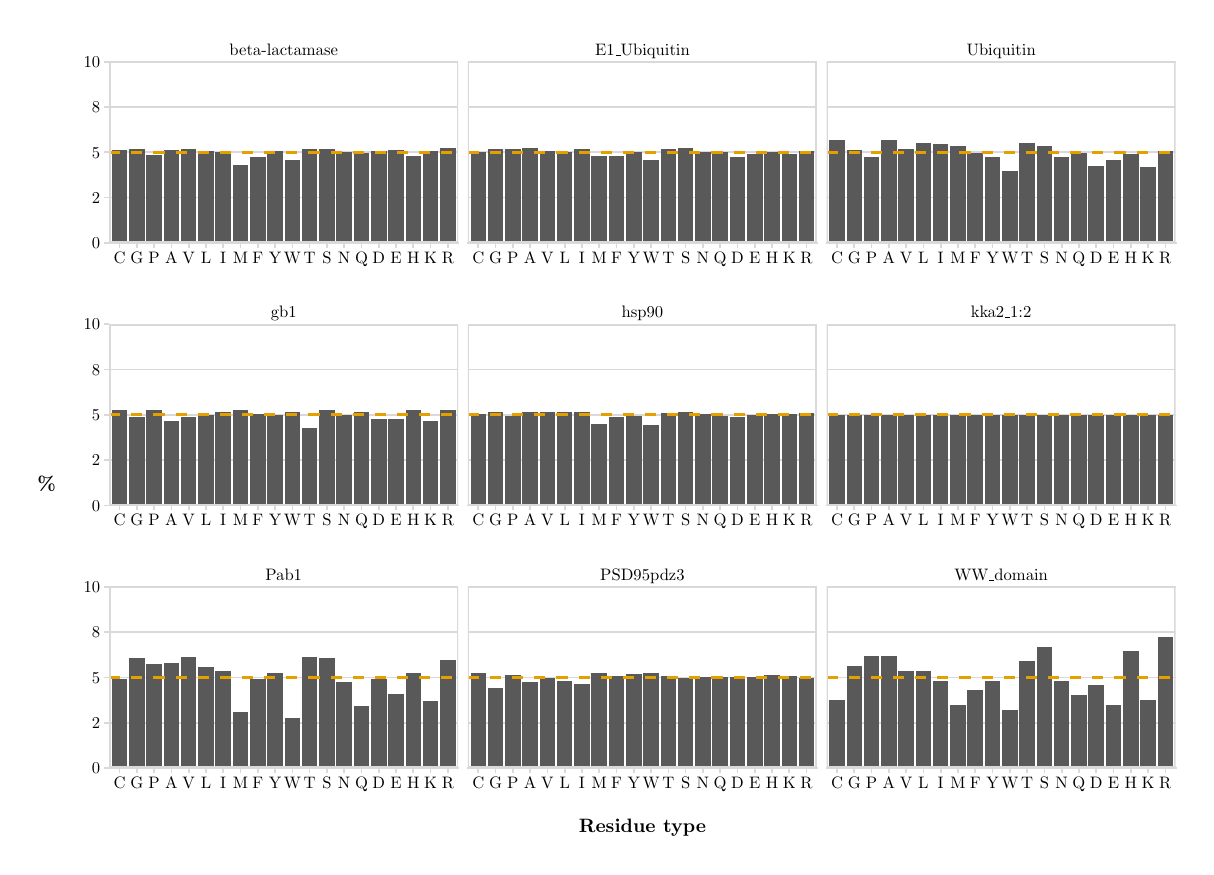
\begin{tikzpicture}[x=1pt,y=1pt]
\definecolor{fillColor}{RGB}{255,255,255}
\path[use as bounding box,fill=fillColor,fill opacity=0.00] (0,0) rectangle (418.34,295.82);
\begin{scope}
\path[clip] ( 29.46,218.05) rectangle (155.58,283.52);
\definecolor{drawColor}{gray}{0.85}

\path[draw=drawColor,line width= 0.6pt,line join=round] ( 29.46,218.05) --
	(155.58,218.05);

\path[draw=drawColor,line width= 0.6pt,line join=round] ( 29.46,234.42) --
	(155.58,234.42);

\path[draw=drawColor,line width= 0.6pt,line join=round] ( 29.46,250.78) --
	(155.58,250.78);

\path[draw=drawColor,line width= 0.6pt,line join=round] ( 29.46,267.15) --
	(155.58,267.15);

\path[draw=drawColor,line width= 0.6pt,line join=round] ( 29.46,283.52) --
	(155.58,283.52);
\definecolor{fillColor}{gray}{0.35}

\path[fill=fillColor] ( 30.39,218.05) rectangle ( 36.01,251.53);

\path[fill=fillColor] ( 36.64,218.05) rectangle ( 42.26,251.89);

\path[fill=fillColor] ( 42.88,218.05) rectangle ( 48.50,249.83);

\path[fill=fillColor] ( 49.13,218.05) rectangle ( 54.75,251.77);

\path[fill=fillColor] ( 55.37,218.05) rectangle ( 60.99,251.89);

\path[fill=fillColor] ( 61.61,218.05) rectangle ( 67.23,251.41);

\path[fill=fillColor] ( 67.86,218.05) rectangle ( 73.48,250.92);

\path[fill=fillColor] ( 74.10,218.05) rectangle ( 79.72,246.07);

\path[fill=fillColor] ( 80.35,218.05) rectangle ( 85.96,249.23);

\path[fill=fillColor] ( 86.59,218.05) rectangle ( 92.21,251.17);

\path[fill=fillColor] ( 92.83,218.05) rectangle ( 98.45,248.13);

\path[fill=fillColor] ( 99.08,218.05) rectangle (104.70,252.14);

\path[fill=fillColor] (105.32,218.05) rectangle (110.94,252.02);

\path[fill=fillColor] (111.56,218.05) rectangle (117.18,250.92);

\path[fill=fillColor] (117.81,218.05) rectangle (123.43,250.56);

\path[fill=fillColor] (124.05,218.05) rectangle (129.67,251.41);

\path[fill=fillColor] (130.30,218.05) rectangle (135.92,251.77);

\path[fill=fillColor] (136.54,218.05) rectangle (142.16,249.59);

\path[fill=fillColor] (142.78,218.05) rectangle (148.40,251.17);

\path[fill=fillColor] (149.03,218.05) rectangle (154.65,252.26);
\definecolor{drawColor}{RGB}{230,159,0}

\path[draw=drawColor,line width= 1.1pt,dash pattern=on 4pt off 4pt ,line join=round] ( 29.46,250.78) -- (155.58,250.78);
\definecolor{drawColor}{gray}{0.85}

\path[draw=drawColor,line width= 1.1pt,line join=round,line cap=round] ( 29.46,218.05) rectangle (155.58,283.52);
\end{scope}
\begin{scope}
\path[clip] ( 29.46,123.17) rectangle (155.58,188.65);
\definecolor{drawColor}{gray}{0.85}

\path[draw=drawColor,line width= 0.6pt,line join=round] ( 29.46,123.17) --
	(155.58,123.17);

\path[draw=drawColor,line width= 0.6pt,line join=round] ( 29.46,139.54) --
	(155.58,139.54);

\path[draw=drawColor,line width= 0.6pt,line join=round] ( 29.46,155.91) --
	(155.58,155.91);

\path[draw=drawColor,line width= 0.6pt,line join=round] ( 29.46,172.28) --
	(155.58,172.28);

\path[draw=drawColor,line width= 0.6pt,line join=round] ( 29.46,188.65) --
	(155.58,188.65);
\definecolor{fillColor}{gray}{0.35}

\path[fill=fillColor] ( 30.39,123.17) rectangle ( 36.01,157.64);

\path[fill=fillColor] ( 36.64,123.17) rectangle ( 42.26,155.08);

\path[fill=fillColor] ( 42.88,123.17) rectangle ( 48.50,157.64);

\path[fill=fillColor] ( 49.13,123.17) rectangle ( 54.75,153.81);

\path[fill=fillColor] ( 55.37,123.17) rectangle ( 60.99,155.08);

\path[fill=fillColor] ( 61.61,123.17) rectangle ( 67.23,155.72);

\path[fill=fillColor] ( 67.86,123.17) rectangle ( 73.48,157.00);

\path[fill=fillColor] ( 74.10,123.17) rectangle ( 79.72,157.64);

\path[fill=fillColor] ( 80.35,123.17) rectangle ( 85.96,156.36);

\path[fill=fillColor] ( 86.59,123.17) rectangle ( 92.21,155.72);

\path[fill=fillColor] ( 92.83,123.17) rectangle ( 98.45,157.00);

\path[fill=fillColor] ( 99.08,123.17) rectangle (104.70,151.25);

\path[fill=fillColor] (105.32,123.17) rectangle (110.94,157.64);

\path[fill=fillColor] (111.56,123.17) rectangle (117.18,155.72);

\path[fill=fillColor] (117.81,123.17) rectangle (123.43,157.00);

\path[fill=fillColor] (124.05,123.17) rectangle (129.67,154.45);

\path[fill=fillColor] (130.30,123.17) rectangle (135.92,154.45);

\path[fill=fillColor] (136.54,123.17) rectangle (142.16,157.64);

\path[fill=fillColor] (142.78,123.17) rectangle (148.40,153.81);

\path[fill=fillColor] (149.03,123.17) rectangle (154.65,157.64);
\definecolor{drawColor}{RGB}{230,159,0}

\path[draw=drawColor,line width= 1.1pt,dash pattern=on 4pt off 4pt ,line join=round] ( 29.46,155.91) -- (155.58,155.91);
\definecolor{drawColor}{gray}{0.85}

\path[draw=drawColor,line width= 1.1pt,line join=round,line cap=round] ( 29.46,123.17) rectangle (155.58,188.65);
\end{scope}
\begin{scope}
\path[clip] ( 29.46, 28.30) rectangle (155.58, 93.78);
\definecolor{drawColor}{gray}{0.85}

\path[draw=drawColor,line width= 0.6pt,line join=round] ( 29.46, 28.30) --
	(155.58, 28.30);

\path[draw=drawColor,line width= 0.6pt,line join=round] ( 29.46, 44.67) --
	(155.58, 44.67);

\path[draw=drawColor,line width= 0.6pt,line join=round] ( 29.46, 61.04) --
	(155.58, 61.04);

\path[draw=drawColor,line width= 0.6pt,line join=round] ( 29.46, 77.41) --
	(155.58, 77.41);

\path[draw=drawColor,line width= 0.6pt,line join=round] ( 29.46, 93.78) --
	(155.58, 93.78);
\definecolor{fillColor}{gray}{0.35}

\path[fill=fillColor] ( 30.39, 28.30) rectangle ( 36.01, 60.51);

\path[fill=fillColor] ( 36.64, 28.30) rectangle ( 42.26, 68.02);

\path[fill=fillColor] ( 42.88, 28.30) rectangle ( 48.50, 65.87);

\path[fill=fillColor] ( 49.13, 28.30) rectangle ( 54.75, 66.41);

\path[fill=fillColor] ( 55.37, 28.30) rectangle ( 60.99, 68.56);

\path[fill=fillColor] ( 61.61, 28.30) rectangle ( 67.23, 64.80);

\path[fill=fillColor] ( 67.86, 28.30) rectangle ( 73.48, 63.19);

\path[fill=fillColor] ( 74.10, 28.30) rectangle ( 79.72, 48.70);

\path[fill=fillColor] ( 80.35, 28.30) rectangle ( 85.96, 60.51);

\path[fill=fillColor] ( 86.59, 28.30) rectangle ( 92.21, 62.65);

\path[fill=fillColor] ( 92.83, 28.30) rectangle ( 98.45, 46.55);

\path[fill=fillColor] ( 99.08, 28.30) rectangle (104.70, 68.56);

\path[fill=fillColor] (105.32, 28.30) rectangle (110.94, 68.02);

\path[fill=fillColor] (111.56, 28.30) rectangle (117.18, 59.43);

\path[fill=fillColor] (117.81, 28.30) rectangle (123.43, 50.84);

\path[fill=fillColor] (124.05, 28.30) rectangle (129.67, 60.51);

\path[fill=fillColor] (130.30, 28.30) rectangle (135.92, 55.14);

\path[fill=fillColor] (136.54, 28.30) rectangle (142.16, 62.65);

\path[fill=fillColor] (142.78, 28.30) rectangle (148.40, 52.46);

\path[fill=fillColor] (149.03, 28.30) rectangle (154.65, 67.48);
\definecolor{drawColor}{RGB}{230,159,0}

\path[draw=drawColor,line width= 1.1pt,dash pattern=on 4pt off 4pt ,line join=round] ( 29.46, 61.04) -- (155.58, 61.04);
\definecolor{drawColor}{gray}{0.85}

\path[draw=drawColor,line width= 1.1pt,line join=round,line cap=round] ( 29.46, 28.30) rectangle (155.58, 93.78);
\end{scope}
\begin{scope}
\path[clip] (159.08,218.05) rectangle (285.21,283.52);
\definecolor{drawColor}{gray}{0.85}

\path[draw=drawColor,line width= 0.6pt,line join=round] (159.08,218.05) --
	(285.21,218.05);

\path[draw=drawColor,line width= 0.6pt,line join=round] (159.08,234.42) --
	(285.21,234.42);

\path[draw=drawColor,line width= 0.6pt,line join=round] (159.08,250.78) --
	(285.21,250.78);

\path[draw=drawColor,line width= 0.6pt,line join=round] (159.08,267.15) --
	(285.21,267.15);

\path[draw=drawColor,line width= 0.6pt,line join=round] (159.08,283.52) --
	(285.21,283.52);
\definecolor{fillColor}{gray}{0.35}

\path[fill=fillColor] (160.02,218.05) rectangle (165.64,250.73);

\path[fill=fillColor] (166.26,218.05) rectangle (171.88,251.87);

\path[fill=fillColor] (172.51,218.05) rectangle (178.13,251.87);

\path[fill=fillColor] (178.75,218.05) rectangle (184.37,252.45);

\path[fill=fillColor] (185.00,218.05) rectangle (190.62,251.30);

\path[fill=fillColor] (191.24,218.05) rectangle (196.86,250.73);

\path[fill=fillColor] (197.48,218.05) rectangle (203.10,251.87);

\path[fill=fillColor] (203.73,218.05) rectangle (209.35,249.58);

\path[fill=fillColor] (209.97,218.05) rectangle (215.59,249.58);

\path[fill=fillColor] (216.22,218.05) rectangle (221.83,250.73);

\path[fill=fillColor] (222.46,218.05) rectangle (228.08,247.86);

\path[fill=fillColor] (228.70,218.05) rectangle (234.32,251.87);

\path[fill=fillColor] (234.95,218.05) rectangle (240.57,252.45);

\path[fill=fillColor] (241.19,218.05) rectangle (246.81,250.73);

\path[fill=fillColor] (247.43,218.05) rectangle (253.05,250.73);

\path[fill=fillColor] (253.68,218.05) rectangle (259.30,249.01);

\path[fill=fillColor] (259.92,218.05) rectangle (265.54,250.15);

\path[fill=fillColor] (266.17,218.05) rectangle (271.79,250.73);

\path[fill=fillColor] (272.41,218.05) rectangle (278.03,250.15);

\path[fill=fillColor] (278.65,218.05) rectangle (284.27,251.30);
\definecolor{drawColor}{RGB}{230,159,0}

\path[draw=drawColor,line width= 1.1pt,dash pattern=on 4pt off 4pt ,line join=round] (159.08,250.78) -- (285.21,250.78);
\definecolor{drawColor}{gray}{0.85}

\path[draw=drawColor,line width= 1.1pt,line join=round,line cap=round] (159.08,218.05) rectangle (285.21,283.52);
\end{scope}
\begin{scope}
\path[clip] (159.08,123.17) rectangle (285.21,188.65);
\definecolor{drawColor}{gray}{0.85}

\path[draw=drawColor,line width= 0.6pt,line join=round] (159.08,123.17) --
	(285.21,123.17);

\path[draw=drawColor,line width= 0.6pt,line join=round] (159.08,139.54) --
	(285.21,139.54);

\path[draw=drawColor,line width= 0.6pt,line join=round] (159.08,155.91) --
	(285.21,155.91);

\path[draw=drawColor,line width= 0.6pt,line join=round] (159.08,172.28) --
	(285.21,172.28);

\path[draw=drawColor,line width= 0.6pt,line join=round] (159.08,188.65) --
	(285.21,188.65);
\definecolor{fillColor}{gray}{0.35}

\path[fill=fillColor] (160.02,123.17) rectangle (165.64,156.14);

\path[fill=fillColor] (166.26,123.17) rectangle (171.88,156.91);

\path[fill=fillColor] (172.51,123.17) rectangle (178.13,155.67);

\path[fill=fillColor] (178.75,123.17) rectangle (184.37,157.07);

\path[fill=fillColor] (185.00,123.17) rectangle (190.62,157.07);

\path[fill=fillColor] (191.24,123.17) rectangle (196.86,157.07);

\path[fill=fillColor] (197.48,123.17) rectangle (203.10,156.91);

\path[fill=fillColor] (203.73,123.17) rectangle (209.35,152.73);

\path[fill=fillColor] (209.97,123.17) rectangle (215.59,155.21);

\path[fill=fillColor] (216.22,123.17) rectangle (221.83,155.52);

\path[fill=fillColor] (222.46,123.17) rectangle (228.08,152.11);

\path[fill=fillColor] (228.70,123.17) rectangle (234.32,156.76);

\path[fill=fillColor] (234.95,123.17) rectangle (240.57,157.07);

\path[fill=fillColor] (241.19,123.17) rectangle (246.81,156.14);

\path[fill=fillColor] (247.43,123.17) rectangle (253.05,155.67);

\path[fill=fillColor] (253.68,123.17) rectangle (259.30,155.21);

\path[fill=fillColor] (259.92,123.17) rectangle (265.54,155.83);

\path[fill=fillColor] (266.17,123.17) rectangle (271.79,156.29);

\path[fill=fillColor] (272.41,123.17) rectangle (278.03,156.29);

\path[fill=fillColor] (278.65,123.17) rectangle (284.27,156.60);
\definecolor{drawColor}{RGB}{230,159,0}

\path[draw=drawColor,line width= 1.1pt,dash pattern=on 4pt off 4pt ,line join=round] (159.08,155.91) -- (285.21,155.91);
\definecolor{drawColor}{gray}{0.85}

\path[draw=drawColor,line width= 1.1pt,line join=round,line cap=round] (159.08,123.17) rectangle (285.21,188.65);
\end{scope}
\begin{scope}
\path[clip] (159.08, 28.30) rectangle (285.21, 93.78);
\definecolor{drawColor}{gray}{0.85}

\path[draw=drawColor,line width= 0.6pt,line join=round] (159.08, 28.30) --
	(285.21, 28.30);

\path[draw=drawColor,line width= 0.6pt,line join=round] (159.08, 44.67) --
	(285.21, 44.67);

\path[draw=drawColor,line width= 0.6pt,line join=round] (159.08, 61.04) --
	(285.21, 61.04);

\path[draw=drawColor,line width= 0.6pt,line join=round] (159.08, 77.41) --
	(285.21, 77.41);

\path[draw=drawColor,line width= 0.6pt,line join=round] (159.08, 93.78) --
	(285.21, 93.78);
\definecolor{fillColor}{gray}{0.35}

\path[fill=fillColor] (160.02, 28.30) rectangle (165.64, 62.77);

\path[fill=fillColor] (166.26, 28.30) rectangle (171.88, 57.37);

\path[fill=fillColor] (172.51, 28.30) rectangle (178.13, 61.93);

\path[fill=fillColor] (178.75, 28.30) rectangle (184.37, 59.44);

\path[fill=fillColor] (185.00, 28.30) rectangle (190.62, 60.69);

\path[fill=fillColor] (191.24, 28.30) rectangle (196.86, 59.86);

\path[fill=fillColor] (197.48, 28.30) rectangle (203.10, 58.61);

\path[fill=fillColor] (203.73, 28.30) rectangle (209.35, 62.77);

\path[fill=fillColor] (209.97, 28.30) rectangle (215.59, 61.52);

\path[fill=fillColor] (216.22, 28.30) rectangle (221.83, 62.35);

\path[fill=fillColor] (222.46, 28.30) rectangle (228.08, 62.77);

\path[fill=fillColor] (228.70, 28.30) rectangle (234.32, 61.52);

\path[fill=fillColor] (234.95, 28.30) rectangle (240.57, 60.69);

\path[fill=fillColor] (241.19, 28.30) rectangle (246.81, 61.10);

\path[fill=fillColor] (247.43, 28.30) rectangle (253.05, 61.10);

\path[fill=fillColor] (253.68, 28.30) rectangle (259.30, 61.10);

\path[fill=fillColor] (259.92, 28.30) rectangle (265.54, 61.10);

\path[fill=fillColor] (266.17, 28.30) rectangle (271.79, 61.93);

\path[fill=fillColor] (272.41, 28.30) rectangle (278.03, 61.52);

\path[fill=fillColor] (278.65, 28.30) rectangle (284.27, 60.69);
\definecolor{drawColor}{RGB}{230,159,0}

\path[draw=drawColor,line width= 1.1pt,dash pattern=on 4pt off 4pt ,line join=round] (159.08, 61.04) -- (285.21, 61.04);
\definecolor{drawColor}{gray}{0.85}

\path[draw=drawColor,line width= 1.1pt,line join=round,line cap=round] (159.08, 28.30) rectangle (285.21, 93.78);
\end{scope}
\begin{scope}
\path[clip] (288.71,218.05) rectangle (414.84,283.52);
\definecolor{drawColor}{gray}{0.85}

\path[draw=drawColor,line width= 0.6pt,line join=round] (288.71,218.05) --
	(414.84,218.05);

\path[draw=drawColor,line width= 0.6pt,line join=round] (288.71,234.42) --
	(414.84,234.42);

\path[draw=drawColor,line width= 0.6pt,line join=round] (288.71,250.78) --
	(414.84,250.78);

\path[draw=drawColor,line width= 0.6pt,line join=round] (288.71,267.15) --
	(414.84,267.15);

\path[draw=drawColor,line width= 0.6pt,line join=round] (288.71,283.52) --
	(414.84,283.52);
\definecolor{fillColor}{gray}{0.35}

\path[fill=fillColor] (289.65,218.05) rectangle (295.27,255.25);

\path[fill=fillColor] (295.89,218.05) rectangle (301.51,251.64);

\path[fill=fillColor] (302.13,218.05) rectangle (307.75,249.05);

\path[fill=fillColor] (308.38,218.05) rectangle (314.00,255.25);

\path[fill=fillColor] (314.62,218.05) rectangle (320.24,252.15);

\path[fill=fillColor] (320.87,218.05) rectangle (326.49,254.22);

\path[fill=fillColor] (327.11,218.05) rectangle (332.73,253.70);

\path[fill=fillColor] (333.35,218.05) rectangle (338.97,253.19);

\path[fill=fillColor] (339.60,218.05) rectangle (345.22,250.60);

\path[fill=fillColor] (345.84,218.05) rectangle (351.46,249.05);

\path[fill=fillColor] (352.08,218.05) rectangle (357.70,243.89);

\path[fill=fillColor] (358.33,218.05) rectangle (363.95,254.22);

\path[fill=fillColor] (364.57,218.05) rectangle (370.19,253.19);

\path[fill=fillColor] (370.82,218.05) rectangle (376.44,249.05);

\path[fill=fillColor] (377.06,218.05) rectangle (382.68,250.60);

\path[fill=fillColor] (383.30,218.05) rectangle (388.92,245.95);

\path[fill=fillColor] (389.55,218.05) rectangle (395.17,248.02);

\path[fill=fillColor] (395.79,218.05) rectangle (401.41,250.09);

\path[fill=fillColor] (402.04,218.05) rectangle (407.66,245.44);

\path[fill=fillColor] (408.28,218.05) rectangle (413.90,251.12);
\definecolor{drawColor}{RGB}{230,159,0}

\path[draw=drawColor,line width= 1.1pt,dash pattern=on 4pt off 4pt ,line join=round] (288.71,250.78) -- (414.84,250.78);
\definecolor{drawColor}{gray}{0.85}

\path[draw=drawColor,line width= 1.1pt,line join=round,line cap=round] (288.71,218.05) rectangle (414.84,283.52);
\end{scope}
\begin{scope}
\path[clip] (288.71,123.17) rectangle (414.84,188.65);
\definecolor{drawColor}{gray}{0.85}

\path[draw=drawColor,line width= 0.6pt,line join=round] (288.71,123.17) --
	(414.84,123.17);

\path[draw=drawColor,line width= 0.6pt,line join=round] (288.71,139.54) --
	(414.84,139.54);

\path[draw=drawColor,line width= 0.6pt,line join=round] (288.71,155.91) --
	(414.84,155.91);

\path[draw=drawColor,line width= 0.6pt,line join=round] (288.71,172.28) --
	(414.84,172.28);

\path[draw=drawColor,line width= 0.6pt,line join=round] (288.71,188.65) --
	(414.84,188.65);
\definecolor{fillColor}{gray}{0.35}

\path[fill=fillColor] (289.65,123.17) rectangle (295.27,155.91);

\path[fill=fillColor] (295.89,123.17) rectangle (301.51,155.91);

\path[fill=fillColor] (302.13,123.17) rectangle (307.75,155.91);

\path[fill=fillColor] (308.38,123.17) rectangle (314.00,155.91);

\path[fill=fillColor] (314.62,123.17) rectangle (320.24,155.91);

\path[fill=fillColor] (320.87,123.17) rectangle (326.49,155.91);

\path[fill=fillColor] (327.11,123.17) rectangle (332.73,155.91);

\path[fill=fillColor] (333.35,123.17) rectangle (338.97,155.91);

\path[fill=fillColor] (339.60,123.17) rectangle (345.22,155.91);

\path[fill=fillColor] (345.84,123.17) rectangle (351.46,155.91);

\path[fill=fillColor] (352.08,123.17) rectangle (357.70,155.91);

\path[fill=fillColor] (358.33,123.17) rectangle (363.95,155.91);

\path[fill=fillColor] (364.57,123.17) rectangle (370.19,155.91);

\path[fill=fillColor] (370.82,123.17) rectangle (376.44,155.91);

\path[fill=fillColor] (377.06,123.17) rectangle (382.68,155.91);

\path[fill=fillColor] (383.30,123.17) rectangle (388.92,155.91);

\path[fill=fillColor] (389.55,123.17) rectangle (395.17,155.91);

\path[fill=fillColor] (395.79,123.17) rectangle (401.41,155.91);

\path[fill=fillColor] (402.04,123.17) rectangle (407.66,155.91);

\path[fill=fillColor] (408.28,123.17) rectangle (413.90,155.91);
\definecolor{drawColor}{RGB}{230,159,0}

\path[draw=drawColor,line width= 1.1pt,dash pattern=on 4pt off 4pt ,line join=round] (288.71,155.91) -- (414.84,155.91);
\definecolor{drawColor}{gray}{0.85}

\path[draw=drawColor,line width= 1.1pt,line join=round,line cap=round] (288.71,123.17) rectangle (414.84,188.65);
\end{scope}
\begin{scope}
\path[clip] (288.71, 28.30) rectangle (414.84, 93.78);
\definecolor{drawColor}{gray}{0.85}

\path[draw=drawColor,line width= 0.6pt,line join=round] (288.71, 28.30) --
	(414.84, 28.30);

\path[draw=drawColor,line width= 0.6pt,line join=round] (288.71, 44.67) --
	(414.84, 44.67);

\path[draw=drawColor,line width= 0.6pt,line join=round] (288.71, 61.04) --
	(414.84, 61.04);

\path[draw=drawColor,line width= 0.6pt,line join=round] (288.71, 77.41) --
	(414.84, 77.41);

\path[draw=drawColor,line width= 0.6pt,line join=round] (288.71, 93.78) --
	(414.84, 93.78);
\definecolor{fillColor}{gray}{0.35}

\path[fill=fillColor] (289.65, 28.30) rectangle (295.27, 52.88);

\path[fill=fillColor] (295.89, 28.30) rectangle (301.51, 65.17);

\path[fill=fillColor] (302.13, 28.30) rectangle (307.75, 68.68);

\path[fill=fillColor] (308.38, 28.30) rectangle (314.00, 68.68);

\path[fill=fillColor] (314.62, 28.30) rectangle (320.24, 63.41);

\path[fill=fillColor] (320.87, 28.30) rectangle (326.49, 63.41);

\path[fill=fillColor] (327.11, 28.30) rectangle (332.73, 59.90);

\path[fill=fillColor] (333.35, 28.30) rectangle (338.97, 51.12);

\path[fill=fillColor] (339.60, 28.30) rectangle (345.22, 56.39);

\path[fill=fillColor] (345.84, 28.30) rectangle (351.46, 59.90);

\path[fill=fillColor] (352.08, 28.30) rectangle (357.70, 49.37);

\path[fill=fillColor] (358.33, 28.30) rectangle (363.95, 66.92);

\path[fill=fillColor] (364.57, 28.30) rectangle (370.19, 72.19);

\path[fill=fillColor] (370.82, 28.30) rectangle (376.44, 59.90);

\path[fill=fillColor] (377.06, 28.30) rectangle (382.68, 54.63);

\path[fill=fillColor] (383.30, 28.30) rectangle (388.92, 58.15);

\path[fill=fillColor] (389.55, 28.30) rectangle (395.17, 51.12);

\path[fill=fillColor] (395.79, 28.30) rectangle (401.41, 70.43);

\path[fill=fillColor] (402.04, 28.30) rectangle (407.66, 52.88);

\path[fill=fillColor] (408.28, 28.30) rectangle (413.90, 75.70);
\definecolor{drawColor}{RGB}{230,159,0}

\path[draw=drawColor,line width= 1.1pt,dash pattern=on 4pt off 4pt ,line join=round] (288.71, 61.04) -- (414.84, 61.04);
\definecolor{drawColor}{gray}{0.85}

\path[draw=drawColor,line width= 1.1pt,line join=round,line cap=round] (288.71, 28.30) rectangle (414.84, 93.78);
\end{scope}
\begin{scope}
\path[clip] ( 29.46, 93.78) rectangle (155.58,102.58);
\definecolor{drawColor}{RGB}{0,0,0}

\node[text=drawColor,anchor=base,inner sep=0pt, outer sep=0pt, scale=  0.60] at ( 92.52, 96.11) {Pab1};
\end{scope}
\begin{scope}
\path[clip] (159.08, 93.78) rectangle (285.21,102.58);
\definecolor{drawColor}{RGB}{0,0,0}

\node[text=drawColor,anchor=base,inner sep=0pt, outer sep=0pt, scale=  0.60] at (222.15, 96.11) {PSD95pdz3};
\end{scope}
\begin{scope}
\path[clip] (288.71, 93.78) rectangle (414.84,102.58);
\definecolor{drawColor}{RGB}{0,0,0}

\node[text=drawColor,anchor=base,inner sep=0pt, outer sep=0pt, scale=  0.60] at (351.77, 96.11) {WW\_domain};
\end{scope}
\begin{scope}
\path[clip] ( 29.46,188.65) rectangle (155.58,197.45);
\definecolor{drawColor}{RGB}{0,0,0}

\node[text=drawColor,anchor=base,inner sep=0pt, outer sep=0pt, scale=  0.60] at ( 92.52,190.99) {gb1};
\end{scope}
\begin{scope}
\path[clip] (159.08,188.65) rectangle (285.21,197.45);
\definecolor{drawColor}{RGB}{0,0,0}

\node[text=drawColor,anchor=base,inner sep=0pt, outer sep=0pt, scale=  0.60] at (222.15,190.99) {hsp90};
\end{scope}
\begin{scope}
\path[clip] (288.71,188.65) rectangle (414.84,197.45);
\definecolor{drawColor}{RGB}{0,0,0}

\node[text=drawColor,anchor=base,inner sep=0pt, outer sep=0pt, scale=  0.60] at (351.77,190.99) {kka2\_1:2};
\end{scope}
\begin{scope}
\path[clip] ( 29.46,283.52) rectangle (155.58,292.32);
\definecolor{drawColor}{RGB}{0,0,0}

\node[text=drawColor,anchor=base,inner sep=0pt, outer sep=0pt, scale=  0.60] at ( 92.52,285.86) {beta-lactamase};
\end{scope}
\begin{scope}
\path[clip] (159.08,283.52) rectangle (285.21,292.32);
\definecolor{drawColor}{RGB}{0,0,0}

\node[text=drawColor,anchor=base,inner sep=0pt, outer sep=0pt, scale=  0.60] at (222.15,285.86) {E1\_Ubiquitin};
\end{scope}
\begin{scope}
\path[clip] (288.71,283.52) rectangle (414.84,292.32);
\definecolor{drawColor}{RGB}{0,0,0}

\node[text=drawColor,anchor=base,inner sep=0pt, outer sep=0pt, scale=  0.60] at (351.77,285.86) {Ubiquitin};
\end{scope}
\begin{scope}
\path[clip] (  0.00,  0.00) rectangle (418.34,295.82);
\definecolor{drawColor}{gray}{0.85}

\path[draw=drawColor,line width= 0.6pt,line join=round,line cap=rect] ( 29.46, 28.30) --
	(155.58, 28.30);
\end{scope}
\begin{scope}
\path[clip] (  0.00,  0.00) rectangle (418.34,295.82);
\definecolor{drawColor}{gray}{0.85}

\path[draw=drawColor,line width= 0.6pt,line join=round] ( 33.20, 26.55) --
	( 33.20, 28.30);

\path[draw=drawColor,line width= 0.6pt,line join=round] ( 39.45, 26.55) --
	( 39.45, 28.30);

\path[draw=drawColor,line width= 0.6pt,line join=round] ( 45.69, 26.55) --
	( 45.69, 28.30);

\path[draw=drawColor,line width= 0.6pt,line join=round] ( 51.94, 26.55) --
	( 51.94, 28.30);

\path[draw=drawColor,line width= 0.6pt,line join=round] ( 58.18, 26.55) --
	( 58.18, 28.30);

\path[draw=drawColor,line width= 0.6pt,line join=round] ( 64.42, 26.55) --
	( 64.42, 28.30);

\path[draw=drawColor,line width= 0.6pt,line join=round] ( 70.67, 26.55) --
	( 70.67, 28.30);

\path[draw=drawColor,line width= 0.6pt,line join=round] ( 76.91, 26.55) --
	( 76.91, 28.30);

\path[draw=drawColor,line width= 0.6pt,line join=round] ( 83.16, 26.55) --
	( 83.16, 28.30);

\path[draw=drawColor,line width= 0.6pt,line join=round] ( 89.40, 26.55) --
	( 89.40, 28.30);

\path[draw=drawColor,line width= 0.6pt,line join=round] ( 95.64, 26.55) --
	( 95.64, 28.30);

\path[draw=drawColor,line width= 0.6pt,line join=round] (101.89, 26.55) --
	(101.89, 28.30);

\path[draw=drawColor,line width= 0.6pt,line join=round] (108.13, 26.55) --
	(108.13, 28.30);

\path[draw=drawColor,line width= 0.6pt,line join=round] (114.37, 26.55) --
	(114.37, 28.30);

\path[draw=drawColor,line width= 0.6pt,line join=round] (120.62, 26.55) --
	(120.62, 28.30);

\path[draw=drawColor,line width= 0.6pt,line join=round] (126.86, 26.55) --
	(126.86, 28.30);

\path[draw=drawColor,line width= 0.6pt,line join=round] (133.11, 26.55) --
	(133.11, 28.30);

\path[draw=drawColor,line width= 0.6pt,line join=round] (139.35, 26.55) --
	(139.35, 28.30);

\path[draw=drawColor,line width= 0.6pt,line join=round] (145.59, 26.55) --
	(145.59, 28.30);

\path[draw=drawColor,line width= 0.6pt,line join=round] (151.84, 26.55) --
	(151.84, 28.30);
\end{scope}
\begin{scope}
\path[clip] (  0.00,  0.00) rectangle (418.34,295.82);
\definecolor{drawColor}{RGB}{0,0,0}

\node[text=drawColor,anchor=base,inner sep=0pt, outer sep=0pt, scale=  0.60] at ( 33.20, 20.92) {C};

\node[text=drawColor,anchor=base,inner sep=0pt, outer sep=0pt, scale=  0.60] at ( 39.45, 20.92) {G};

\node[text=drawColor,anchor=base,inner sep=0pt, outer sep=0pt, scale=  0.60] at ( 45.69, 20.92) {P};

\node[text=drawColor,anchor=base,inner sep=0pt, outer sep=0pt, scale=  0.60] at ( 51.94, 20.92) {A};

\node[text=drawColor,anchor=base,inner sep=0pt, outer sep=0pt, scale=  0.60] at ( 58.18, 20.92) {V};

\node[text=drawColor,anchor=base,inner sep=0pt, outer sep=0pt, scale=  0.60] at ( 64.42, 20.92) {L};

\node[text=drawColor,anchor=base,inner sep=0pt, outer sep=0pt, scale=  0.60] at ( 70.67, 20.92) {I};

\node[text=drawColor,anchor=base,inner sep=0pt, outer sep=0pt, scale=  0.60] at ( 76.91, 20.92) {M};

\node[text=drawColor,anchor=base,inner sep=0pt, outer sep=0pt, scale=  0.60] at ( 83.16, 20.92) {F};

\node[text=drawColor,anchor=base,inner sep=0pt, outer sep=0pt, scale=  0.60] at ( 89.40, 20.92) {Y};

\node[text=drawColor,anchor=base,inner sep=0pt, outer sep=0pt, scale=  0.60] at ( 95.64, 20.92) {W};

\node[text=drawColor,anchor=base,inner sep=0pt, outer sep=0pt, scale=  0.60] at (101.89, 20.92) {T};

\node[text=drawColor,anchor=base,inner sep=0pt, outer sep=0pt, scale=  0.60] at (108.13, 20.92) {S};

\node[text=drawColor,anchor=base,inner sep=0pt, outer sep=0pt, scale=  0.60] at (114.37, 20.92) {N};

\node[text=drawColor,anchor=base,inner sep=0pt, outer sep=0pt, scale=  0.60] at (120.62, 20.92) {Q};

\node[text=drawColor,anchor=base,inner sep=0pt, outer sep=0pt, scale=  0.60] at (126.86, 20.92) {D};

\node[text=drawColor,anchor=base,inner sep=0pt, outer sep=0pt, scale=  0.60] at (133.11, 20.92) {E};

\node[text=drawColor,anchor=base,inner sep=0pt, outer sep=0pt, scale=  0.60] at (139.35, 20.92) {H};

\node[text=drawColor,anchor=base,inner sep=0pt, outer sep=0pt, scale=  0.60] at (145.59, 20.92) {K};

\node[text=drawColor,anchor=base,inner sep=0pt, outer sep=0pt, scale=  0.60] at (151.84, 20.92) {R};
\end{scope}
\begin{scope}
\path[clip] (  0.00,  0.00) rectangle (418.34,295.82);
\definecolor{drawColor}{gray}{0.85}

\path[draw=drawColor,line width= 0.6pt,line join=round,line cap=rect] (159.08, 28.30) --
	(285.21, 28.30);
\end{scope}
\begin{scope}
\path[clip] (  0.00,  0.00) rectangle (418.34,295.82);
\definecolor{drawColor}{gray}{0.85}

\path[draw=drawColor,line width= 0.6pt,line join=round] (162.83, 26.55) --
	(162.83, 28.30);

\path[draw=drawColor,line width= 0.6pt,line join=round] (169.07, 26.55) --
	(169.07, 28.30);

\path[draw=drawColor,line width= 0.6pt,line join=round] (175.32, 26.55) --
	(175.32, 28.30);

\path[draw=drawColor,line width= 0.6pt,line join=round] (181.56, 26.55) --
	(181.56, 28.30);

\path[draw=drawColor,line width= 0.6pt,line join=round] (187.81, 26.55) --
	(187.81, 28.30);

\path[draw=drawColor,line width= 0.6pt,line join=round] (194.05, 26.55) --
	(194.05, 28.30);

\path[draw=drawColor,line width= 0.6pt,line join=round] (200.29, 26.55) --
	(200.29, 28.30);

\path[draw=drawColor,line width= 0.6pt,line join=round] (206.54, 26.55) --
	(206.54, 28.30);

\path[draw=drawColor,line width= 0.6pt,line join=round] (212.78, 26.55) --
	(212.78, 28.30);

\path[draw=drawColor,line width= 0.6pt,line join=round] (219.02, 26.55) --
	(219.02, 28.30);

\path[draw=drawColor,line width= 0.6pt,line join=round] (225.27, 26.55) --
	(225.27, 28.30);

\path[draw=drawColor,line width= 0.6pt,line join=round] (231.51, 26.55) --
	(231.51, 28.30);

\path[draw=drawColor,line width= 0.6pt,line join=round] (237.76, 26.55) --
	(237.76, 28.30);

\path[draw=drawColor,line width= 0.6pt,line join=round] (244.00, 26.55) --
	(244.00, 28.30);

\path[draw=drawColor,line width= 0.6pt,line join=round] (250.24, 26.55) --
	(250.24, 28.30);

\path[draw=drawColor,line width= 0.6pt,line join=round] (256.49, 26.55) --
	(256.49, 28.30);

\path[draw=drawColor,line width= 0.6pt,line join=round] (262.73, 26.55) --
	(262.73, 28.30);

\path[draw=drawColor,line width= 0.6pt,line join=round] (268.98, 26.55) --
	(268.98, 28.30);

\path[draw=drawColor,line width= 0.6pt,line join=round] (275.22, 26.55) --
	(275.22, 28.30);

\path[draw=drawColor,line width= 0.6pt,line join=round] (281.46, 26.55) --
	(281.46, 28.30);
\end{scope}
\begin{scope}
\path[clip] (  0.00,  0.00) rectangle (418.34,295.82);
\definecolor{drawColor}{RGB}{0,0,0}

\node[text=drawColor,anchor=base,inner sep=0pt, outer sep=0pt, scale=  0.60] at (162.83, 20.92) {C};

\node[text=drawColor,anchor=base,inner sep=0pt, outer sep=0pt, scale=  0.60] at (169.07, 20.92) {G};

\node[text=drawColor,anchor=base,inner sep=0pt, outer sep=0pt, scale=  0.60] at (175.32, 20.92) {P};

\node[text=drawColor,anchor=base,inner sep=0pt, outer sep=0pt, scale=  0.60] at (181.56, 20.92) {A};

\node[text=drawColor,anchor=base,inner sep=0pt, outer sep=0pt, scale=  0.60] at (187.81, 20.92) {V};

\node[text=drawColor,anchor=base,inner sep=0pt, outer sep=0pt, scale=  0.60] at (194.05, 20.92) {L};

\node[text=drawColor,anchor=base,inner sep=0pt, outer sep=0pt, scale=  0.60] at (200.29, 20.92) {I};

\node[text=drawColor,anchor=base,inner sep=0pt, outer sep=0pt, scale=  0.60] at (206.54, 20.92) {M};

\node[text=drawColor,anchor=base,inner sep=0pt, outer sep=0pt, scale=  0.60] at (212.78, 20.92) {F};

\node[text=drawColor,anchor=base,inner sep=0pt, outer sep=0pt, scale=  0.60] at (219.02, 20.92) {Y};

\node[text=drawColor,anchor=base,inner sep=0pt, outer sep=0pt, scale=  0.60] at (225.27, 20.92) {W};

\node[text=drawColor,anchor=base,inner sep=0pt, outer sep=0pt, scale=  0.60] at (231.51, 20.92) {T};

\node[text=drawColor,anchor=base,inner sep=0pt, outer sep=0pt, scale=  0.60] at (237.76, 20.92) {S};

\node[text=drawColor,anchor=base,inner sep=0pt, outer sep=0pt, scale=  0.60] at (244.00, 20.92) {N};

\node[text=drawColor,anchor=base,inner sep=0pt, outer sep=0pt, scale=  0.60] at (250.24, 20.92) {Q};

\node[text=drawColor,anchor=base,inner sep=0pt, outer sep=0pt, scale=  0.60] at (256.49, 20.92) {D};

\node[text=drawColor,anchor=base,inner sep=0pt, outer sep=0pt, scale=  0.60] at (262.73, 20.92) {E};

\node[text=drawColor,anchor=base,inner sep=0pt, outer sep=0pt, scale=  0.60] at (268.98, 20.92) {H};

\node[text=drawColor,anchor=base,inner sep=0pt, outer sep=0pt, scale=  0.60] at (275.22, 20.92) {K};

\node[text=drawColor,anchor=base,inner sep=0pt, outer sep=0pt, scale=  0.60] at (281.46, 20.92) {R};
\end{scope}
\begin{scope}
\path[clip] (  0.00,  0.00) rectangle (418.34,295.82);
\definecolor{drawColor}{gray}{0.85}

\path[draw=drawColor,line width= 0.6pt,line join=round,line cap=rect] (288.71, 28.30) --
	(414.84, 28.30);
\end{scope}
\begin{scope}
\path[clip] (  0.00,  0.00) rectangle (418.34,295.82);
\definecolor{drawColor}{gray}{0.85}

\path[draw=drawColor,line width= 0.6pt,line join=round] (292.46, 26.55) --
	(292.46, 28.30);

\path[draw=drawColor,line width= 0.6pt,line join=round] (298.70, 26.55) --
	(298.70, 28.30);

\path[draw=drawColor,line width= 0.6pt,line join=round] (304.94, 26.55) --
	(304.94, 28.30);

\path[draw=drawColor,line width= 0.6pt,line join=round] (311.19, 26.55) --
	(311.19, 28.30);

\path[draw=drawColor,line width= 0.6pt,line join=round] (317.43, 26.55) --
	(317.43, 28.30);

\path[draw=drawColor,line width= 0.6pt,line join=round] (323.68, 26.55) --
	(323.68, 28.30);

\path[draw=drawColor,line width= 0.6pt,line join=round] (329.92, 26.55) --
	(329.92, 28.30);

\path[draw=drawColor,line width= 0.6pt,line join=round] (336.16, 26.55) --
	(336.16, 28.30);

\path[draw=drawColor,line width= 0.6pt,line join=round] (342.41, 26.55) --
	(342.41, 28.30);

\path[draw=drawColor,line width= 0.6pt,line join=round] (348.65, 26.55) --
	(348.65, 28.30);

\path[draw=drawColor,line width= 0.6pt,line join=round] (354.89, 26.55) --
	(354.89, 28.30);

\path[draw=drawColor,line width= 0.6pt,line join=round] (361.14, 26.55) --
	(361.14, 28.30);

\path[draw=drawColor,line width= 0.6pt,line join=round] (367.38, 26.55) --
	(367.38, 28.30);

\path[draw=drawColor,line width= 0.6pt,line join=round] (373.63, 26.55) --
	(373.63, 28.30);

\path[draw=drawColor,line width= 0.6pt,line join=round] (379.87, 26.55) --
	(379.87, 28.30);

\path[draw=drawColor,line width= 0.6pt,line join=round] (386.11, 26.55) --
	(386.11, 28.30);

\path[draw=drawColor,line width= 0.6pt,line join=round] (392.36, 26.55) --
	(392.36, 28.30);

\path[draw=drawColor,line width= 0.6pt,line join=round] (398.60, 26.55) --
	(398.60, 28.30);

\path[draw=drawColor,line width= 0.6pt,line join=round] (404.85, 26.55) --
	(404.85, 28.30);

\path[draw=drawColor,line width= 0.6pt,line join=round] (411.09, 26.55) --
	(411.09, 28.30);
\end{scope}
\begin{scope}
\path[clip] (  0.00,  0.00) rectangle (418.34,295.82);
\definecolor{drawColor}{RGB}{0,0,0}

\node[text=drawColor,anchor=base,inner sep=0pt, outer sep=0pt, scale=  0.60] at (292.46, 20.92) {C};

\node[text=drawColor,anchor=base,inner sep=0pt, outer sep=0pt, scale=  0.60] at (298.70, 20.92) {G};

\node[text=drawColor,anchor=base,inner sep=0pt, outer sep=0pt, scale=  0.60] at (304.94, 20.92) {P};

\node[text=drawColor,anchor=base,inner sep=0pt, outer sep=0pt, scale=  0.60] at (311.19, 20.92) {A};

\node[text=drawColor,anchor=base,inner sep=0pt, outer sep=0pt, scale=  0.60] at (317.43, 20.92) {V};

\node[text=drawColor,anchor=base,inner sep=0pt, outer sep=0pt, scale=  0.60] at (323.68, 20.92) {L};

\node[text=drawColor,anchor=base,inner sep=0pt, outer sep=0pt, scale=  0.60] at (329.92, 20.92) {I};

\node[text=drawColor,anchor=base,inner sep=0pt, outer sep=0pt, scale=  0.60] at (336.16, 20.92) {M};

\node[text=drawColor,anchor=base,inner sep=0pt, outer sep=0pt, scale=  0.60] at (342.41, 20.92) {F};

\node[text=drawColor,anchor=base,inner sep=0pt, outer sep=0pt, scale=  0.60] at (348.65, 20.92) {Y};

\node[text=drawColor,anchor=base,inner sep=0pt, outer sep=0pt, scale=  0.60] at (354.89, 20.92) {W};

\node[text=drawColor,anchor=base,inner sep=0pt, outer sep=0pt, scale=  0.60] at (361.14, 20.92) {T};

\node[text=drawColor,anchor=base,inner sep=0pt, outer sep=0pt, scale=  0.60] at (367.38, 20.92) {S};

\node[text=drawColor,anchor=base,inner sep=0pt, outer sep=0pt, scale=  0.60] at (373.63, 20.92) {N};

\node[text=drawColor,anchor=base,inner sep=0pt, outer sep=0pt, scale=  0.60] at (379.87, 20.92) {Q};

\node[text=drawColor,anchor=base,inner sep=0pt, outer sep=0pt, scale=  0.60] at (386.11, 20.92) {D};

\node[text=drawColor,anchor=base,inner sep=0pt, outer sep=0pt, scale=  0.60] at (392.36, 20.92) {E};

\node[text=drawColor,anchor=base,inner sep=0pt, outer sep=0pt, scale=  0.60] at (398.60, 20.92) {H};

\node[text=drawColor,anchor=base,inner sep=0pt, outer sep=0pt, scale=  0.60] at (404.85, 20.92) {K};

\node[text=drawColor,anchor=base,inner sep=0pt, outer sep=0pt, scale=  0.60] at (411.09, 20.92) {R};
\end{scope}
\begin{scope}
\path[clip] (  0.00,  0.00) rectangle (418.34,295.82);
\definecolor{drawColor}{gray}{0.85}

\path[draw=drawColor,line width= 0.6pt,line join=round,line cap=rect] ( 29.46,123.17) --
	(155.58,123.17);
\end{scope}
\begin{scope}
\path[clip] (  0.00,  0.00) rectangle (418.34,295.82);
\definecolor{drawColor}{gray}{0.85}

\path[draw=drawColor,line width= 0.6pt,line join=round] ( 33.20,121.42) --
	( 33.20,123.17);

\path[draw=drawColor,line width= 0.6pt,line join=round] ( 39.45,121.42) --
	( 39.45,123.17);

\path[draw=drawColor,line width= 0.6pt,line join=round] ( 45.69,121.42) --
	( 45.69,123.17);

\path[draw=drawColor,line width= 0.6pt,line join=round] ( 51.94,121.42) --
	( 51.94,123.17);

\path[draw=drawColor,line width= 0.6pt,line join=round] ( 58.18,121.42) --
	( 58.18,123.17);

\path[draw=drawColor,line width= 0.6pt,line join=round] ( 64.42,121.42) --
	( 64.42,123.17);

\path[draw=drawColor,line width= 0.6pt,line join=round] ( 70.67,121.42) --
	( 70.67,123.17);

\path[draw=drawColor,line width= 0.6pt,line join=round] ( 76.91,121.42) --
	( 76.91,123.17);

\path[draw=drawColor,line width= 0.6pt,line join=round] ( 83.16,121.42) --
	( 83.16,123.17);

\path[draw=drawColor,line width= 0.6pt,line join=round] ( 89.40,121.42) --
	( 89.40,123.17);

\path[draw=drawColor,line width= 0.6pt,line join=round] ( 95.64,121.42) --
	( 95.64,123.17);

\path[draw=drawColor,line width= 0.6pt,line join=round] (101.89,121.42) --
	(101.89,123.17);

\path[draw=drawColor,line width= 0.6pt,line join=round] (108.13,121.42) --
	(108.13,123.17);

\path[draw=drawColor,line width= 0.6pt,line join=round] (114.37,121.42) --
	(114.37,123.17);

\path[draw=drawColor,line width= 0.6pt,line join=round] (120.62,121.42) --
	(120.62,123.17);

\path[draw=drawColor,line width= 0.6pt,line join=round] (126.86,121.42) --
	(126.86,123.17);

\path[draw=drawColor,line width= 0.6pt,line join=round] (133.11,121.42) --
	(133.11,123.17);

\path[draw=drawColor,line width= 0.6pt,line join=round] (139.35,121.42) --
	(139.35,123.17);

\path[draw=drawColor,line width= 0.6pt,line join=round] (145.59,121.42) --
	(145.59,123.17);

\path[draw=drawColor,line width= 0.6pt,line join=round] (151.84,121.42) --
	(151.84,123.17);
\end{scope}
\begin{scope}
\path[clip] (  0.00,  0.00) rectangle (418.34,295.82);
\definecolor{drawColor}{RGB}{0,0,0}

\node[text=drawColor,anchor=base,inner sep=0pt, outer sep=0pt, scale=  0.60] at ( 33.20,115.79) {C};

\node[text=drawColor,anchor=base,inner sep=0pt, outer sep=0pt, scale=  0.60] at ( 39.45,115.79) {G};

\node[text=drawColor,anchor=base,inner sep=0pt, outer sep=0pt, scale=  0.60] at ( 45.69,115.79) {P};

\node[text=drawColor,anchor=base,inner sep=0pt, outer sep=0pt, scale=  0.60] at ( 51.94,115.79) {A};

\node[text=drawColor,anchor=base,inner sep=0pt, outer sep=0pt, scale=  0.60] at ( 58.18,115.79) {V};

\node[text=drawColor,anchor=base,inner sep=0pt, outer sep=0pt, scale=  0.60] at ( 64.42,115.79) {L};

\node[text=drawColor,anchor=base,inner sep=0pt, outer sep=0pt, scale=  0.60] at ( 70.67,115.79) {I};

\node[text=drawColor,anchor=base,inner sep=0pt, outer sep=0pt, scale=  0.60] at ( 76.91,115.79) {M};

\node[text=drawColor,anchor=base,inner sep=0pt, outer sep=0pt, scale=  0.60] at ( 83.16,115.79) {F};

\node[text=drawColor,anchor=base,inner sep=0pt, outer sep=0pt, scale=  0.60] at ( 89.40,115.79) {Y};

\node[text=drawColor,anchor=base,inner sep=0pt, outer sep=0pt, scale=  0.60] at ( 95.64,115.79) {W};

\node[text=drawColor,anchor=base,inner sep=0pt, outer sep=0pt, scale=  0.60] at (101.89,115.79) {T};

\node[text=drawColor,anchor=base,inner sep=0pt, outer sep=0pt, scale=  0.60] at (108.13,115.79) {S};

\node[text=drawColor,anchor=base,inner sep=0pt, outer sep=0pt, scale=  0.60] at (114.37,115.79) {N};

\node[text=drawColor,anchor=base,inner sep=0pt, outer sep=0pt, scale=  0.60] at (120.62,115.79) {Q};

\node[text=drawColor,anchor=base,inner sep=0pt, outer sep=0pt, scale=  0.60] at (126.86,115.79) {D};

\node[text=drawColor,anchor=base,inner sep=0pt, outer sep=0pt, scale=  0.60] at (133.11,115.79) {E};

\node[text=drawColor,anchor=base,inner sep=0pt, outer sep=0pt, scale=  0.60] at (139.35,115.79) {H};

\node[text=drawColor,anchor=base,inner sep=0pt, outer sep=0pt, scale=  0.60] at (145.59,115.79) {K};

\node[text=drawColor,anchor=base,inner sep=0pt, outer sep=0pt, scale=  0.60] at (151.84,115.79) {R};
\end{scope}
\begin{scope}
\path[clip] (  0.00,  0.00) rectangle (418.34,295.82);
\definecolor{drawColor}{gray}{0.85}

\path[draw=drawColor,line width= 0.6pt,line join=round,line cap=rect] (159.08,123.17) --
	(285.21,123.17);
\end{scope}
\begin{scope}
\path[clip] (  0.00,  0.00) rectangle (418.34,295.82);
\definecolor{drawColor}{gray}{0.85}

\path[draw=drawColor,line width= 0.6pt,line join=round] (162.83,121.42) --
	(162.83,123.17);

\path[draw=drawColor,line width= 0.6pt,line join=round] (169.07,121.42) --
	(169.07,123.17);

\path[draw=drawColor,line width= 0.6pt,line join=round] (175.32,121.42) --
	(175.32,123.17);

\path[draw=drawColor,line width= 0.6pt,line join=round] (181.56,121.42) --
	(181.56,123.17);

\path[draw=drawColor,line width= 0.6pt,line join=round] (187.81,121.42) --
	(187.81,123.17);

\path[draw=drawColor,line width= 0.6pt,line join=round] (194.05,121.42) --
	(194.05,123.17);

\path[draw=drawColor,line width= 0.6pt,line join=round] (200.29,121.42) --
	(200.29,123.17);

\path[draw=drawColor,line width= 0.6pt,line join=round] (206.54,121.42) --
	(206.54,123.17);

\path[draw=drawColor,line width= 0.6pt,line join=round] (212.78,121.42) --
	(212.78,123.17);

\path[draw=drawColor,line width= 0.6pt,line join=round] (219.02,121.42) --
	(219.02,123.17);

\path[draw=drawColor,line width= 0.6pt,line join=round] (225.27,121.42) --
	(225.27,123.17);

\path[draw=drawColor,line width= 0.6pt,line join=round] (231.51,121.42) --
	(231.51,123.17);

\path[draw=drawColor,line width= 0.6pt,line join=round] (237.76,121.42) --
	(237.76,123.17);

\path[draw=drawColor,line width= 0.6pt,line join=round] (244.00,121.42) --
	(244.00,123.17);

\path[draw=drawColor,line width= 0.6pt,line join=round] (250.24,121.42) --
	(250.24,123.17);

\path[draw=drawColor,line width= 0.6pt,line join=round] (256.49,121.42) --
	(256.49,123.17);

\path[draw=drawColor,line width= 0.6pt,line join=round] (262.73,121.42) --
	(262.73,123.17);

\path[draw=drawColor,line width= 0.6pt,line join=round] (268.98,121.42) --
	(268.98,123.17);

\path[draw=drawColor,line width= 0.6pt,line join=round] (275.22,121.42) --
	(275.22,123.17);

\path[draw=drawColor,line width= 0.6pt,line join=round] (281.46,121.42) --
	(281.46,123.17);
\end{scope}
\begin{scope}
\path[clip] (  0.00,  0.00) rectangle (418.34,295.82);
\definecolor{drawColor}{RGB}{0,0,0}

\node[text=drawColor,anchor=base,inner sep=0pt, outer sep=0pt, scale=  0.60] at (162.83,115.79) {C};

\node[text=drawColor,anchor=base,inner sep=0pt, outer sep=0pt, scale=  0.60] at (169.07,115.79) {G};

\node[text=drawColor,anchor=base,inner sep=0pt, outer sep=0pt, scale=  0.60] at (175.32,115.79) {P};

\node[text=drawColor,anchor=base,inner sep=0pt, outer sep=0pt, scale=  0.60] at (181.56,115.79) {A};

\node[text=drawColor,anchor=base,inner sep=0pt, outer sep=0pt, scale=  0.60] at (187.81,115.79) {V};

\node[text=drawColor,anchor=base,inner sep=0pt, outer sep=0pt, scale=  0.60] at (194.05,115.79) {L};

\node[text=drawColor,anchor=base,inner sep=0pt, outer sep=0pt, scale=  0.60] at (200.29,115.79) {I};

\node[text=drawColor,anchor=base,inner sep=0pt, outer sep=0pt, scale=  0.60] at (206.54,115.79) {M};

\node[text=drawColor,anchor=base,inner sep=0pt, outer sep=0pt, scale=  0.60] at (212.78,115.79) {F};

\node[text=drawColor,anchor=base,inner sep=0pt, outer sep=0pt, scale=  0.60] at (219.02,115.79) {Y};

\node[text=drawColor,anchor=base,inner sep=0pt, outer sep=0pt, scale=  0.60] at (225.27,115.79) {W};

\node[text=drawColor,anchor=base,inner sep=0pt, outer sep=0pt, scale=  0.60] at (231.51,115.79) {T};

\node[text=drawColor,anchor=base,inner sep=0pt, outer sep=0pt, scale=  0.60] at (237.76,115.79) {S};

\node[text=drawColor,anchor=base,inner sep=0pt, outer sep=0pt, scale=  0.60] at (244.00,115.79) {N};

\node[text=drawColor,anchor=base,inner sep=0pt, outer sep=0pt, scale=  0.60] at (250.24,115.79) {Q};

\node[text=drawColor,anchor=base,inner sep=0pt, outer sep=0pt, scale=  0.60] at (256.49,115.79) {D};

\node[text=drawColor,anchor=base,inner sep=0pt, outer sep=0pt, scale=  0.60] at (262.73,115.79) {E};

\node[text=drawColor,anchor=base,inner sep=0pt, outer sep=0pt, scale=  0.60] at (268.98,115.79) {H};

\node[text=drawColor,anchor=base,inner sep=0pt, outer sep=0pt, scale=  0.60] at (275.22,115.79) {K};

\node[text=drawColor,anchor=base,inner sep=0pt, outer sep=0pt, scale=  0.60] at (281.46,115.79) {R};
\end{scope}
\begin{scope}
\path[clip] (  0.00,  0.00) rectangle (418.34,295.82);
\definecolor{drawColor}{gray}{0.85}

\path[draw=drawColor,line width= 0.6pt,line join=round,line cap=rect] (288.71,123.17) --
	(414.84,123.17);
\end{scope}
\begin{scope}
\path[clip] (  0.00,  0.00) rectangle (418.34,295.82);
\definecolor{drawColor}{gray}{0.85}

\path[draw=drawColor,line width= 0.6pt,line join=round] (292.46,121.42) --
	(292.46,123.17);

\path[draw=drawColor,line width= 0.6pt,line join=round] (298.70,121.42) --
	(298.70,123.17);

\path[draw=drawColor,line width= 0.6pt,line join=round] (304.94,121.42) --
	(304.94,123.17);

\path[draw=drawColor,line width= 0.6pt,line join=round] (311.19,121.42) --
	(311.19,123.17);

\path[draw=drawColor,line width= 0.6pt,line join=round] (317.43,121.42) --
	(317.43,123.17);

\path[draw=drawColor,line width= 0.6pt,line join=round] (323.68,121.42) --
	(323.68,123.17);

\path[draw=drawColor,line width= 0.6pt,line join=round] (329.92,121.42) --
	(329.92,123.17);

\path[draw=drawColor,line width= 0.6pt,line join=round] (336.16,121.42) --
	(336.16,123.17);

\path[draw=drawColor,line width= 0.6pt,line join=round] (342.41,121.42) --
	(342.41,123.17);

\path[draw=drawColor,line width= 0.6pt,line join=round] (348.65,121.42) --
	(348.65,123.17);

\path[draw=drawColor,line width= 0.6pt,line join=round] (354.89,121.42) --
	(354.89,123.17);

\path[draw=drawColor,line width= 0.6pt,line join=round] (361.14,121.42) --
	(361.14,123.17);

\path[draw=drawColor,line width= 0.6pt,line join=round] (367.38,121.42) --
	(367.38,123.17);

\path[draw=drawColor,line width= 0.6pt,line join=round] (373.63,121.42) --
	(373.63,123.17);

\path[draw=drawColor,line width= 0.6pt,line join=round] (379.87,121.42) --
	(379.87,123.17);

\path[draw=drawColor,line width= 0.6pt,line join=round] (386.11,121.42) --
	(386.11,123.17);

\path[draw=drawColor,line width= 0.6pt,line join=round] (392.36,121.42) --
	(392.36,123.17);

\path[draw=drawColor,line width= 0.6pt,line join=round] (398.60,121.42) --
	(398.60,123.17);

\path[draw=drawColor,line width= 0.6pt,line join=round] (404.85,121.42) --
	(404.85,123.17);

\path[draw=drawColor,line width= 0.6pt,line join=round] (411.09,121.42) --
	(411.09,123.17);
\end{scope}
\begin{scope}
\path[clip] (  0.00,  0.00) rectangle (418.34,295.82);
\definecolor{drawColor}{RGB}{0,0,0}

\node[text=drawColor,anchor=base,inner sep=0pt, outer sep=0pt, scale=  0.60] at (292.46,115.79) {C};

\node[text=drawColor,anchor=base,inner sep=0pt, outer sep=0pt, scale=  0.60] at (298.70,115.79) {G};

\node[text=drawColor,anchor=base,inner sep=0pt, outer sep=0pt, scale=  0.60] at (304.94,115.79) {P};

\node[text=drawColor,anchor=base,inner sep=0pt, outer sep=0pt, scale=  0.60] at (311.19,115.79) {A};

\node[text=drawColor,anchor=base,inner sep=0pt, outer sep=0pt, scale=  0.60] at (317.43,115.79) {V};

\node[text=drawColor,anchor=base,inner sep=0pt, outer sep=0pt, scale=  0.60] at (323.68,115.79) {L};

\node[text=drawColor,anchor=base,inner sep=0pt, outer sep=0pt, scale=  0.60] at (329.92,115.79) {I};

\node[text=drawColor,anchor=base,inner sep=0pt, outer sep=0pt, scale=  0.60] at (336.16,115.79) {M};

\node[text=drawColor,anchor=base,inner sep=0pt, outer sep=0pt, scale=  0.60] at (342.41,115.79) {F};

\node[text=drawColor,anchor=base,inner sep=0pt, outer sep=0pt, scale=  0.60] at (348.65,115.79) {Y};

\node[text=drawColor,anchor=base,inner sep=0pt, outer sep=0pt, scale=  0.60] at (354.89,115.79) {W};

\node[text=drawColor,anchor=base,inner sep=0pt, outer sep=0pt, scale=  0.60] at (361.14,115.79) {T};

\node[text=drawColor,anchor=base,inner sep=0pt, outer sep=0pt, scale=  0.60] at (367.38,115.79) {S};

\node[text=drawColor,anchor=base,inner sep=0pt, outer sep=0pt, scale=  0.60] at (373.63,115.79) {N};

\node[text=drawColor,anchor=base,inner sep=0pt, outer sep=0pt, scale=  0.60] at (379.87,115.79) {Q};

\node[text=drawColor,anchor=base,inner sep=0pt, outer sep=0pt, scale=  0.60] at (386.11,115.79) {D};

\node[text=drawColor,anchor=base,inner sep=0pt, outer sep=0pt, scale=  0.60] at (392.36,115.79) {E};

\node[text=drawColor,anchor=base,inner sep=0pt, outer sep=0pt, scale=  0.60] at (398.60,115.79) {H};

\node[text=drawColor,anchor=base,inner sep=0pt, outer sep=0pt, scale=  0.60] at (404.85,115.79) {K};

\node[text=drawColor,anchor=base,inner sep=0pt, outer sep=0pt, scale=  0.60] at (411.09,115.79) {R};
\end{scope}
\begin{scope}
\path[clip] (  0.00,  0.00) rectangle (418.34,295.82);
\definecolor{drawColor}{gray}{0.85}

\path[draw=drawColor,line width= 0.6pt,line join=round,line cap=rect] ( 29.46,218.05) --
	(155.58,218.05);
\end{scope}
\begin{scope}
\path[clip] (  0.00,  0.00) rectangle (418.34,295.82);
\definecolor{drawColor}{gray}{0.85}

\path[draw=drawColor,line width= 0.6pt,line join=round] ( 33.20,216.30) --
	( 33.20,218.05);

\path[draw=drawColor,line width= 0.6pt,line join=round] ( 39.45,216.30) --
	( 39.45,218.05);

\path[draw=drawColor,line width= 0.6pt,line join=round] ( 45.69,216.30) --
	( 45.69,218.05);

\path[draw=drawColor,line width= 0.6pt,line join=round] ( 51.94,216.30) --
	( 51.94,218.05);

\path[draw=drawColor,line width= 0.6pt,line join=round] ( 58.18,216.30) --
	( 58.18,218.05);

\path[draw=drawColor,line width= 0.6pt,line join=round] ( 64.42,216.30) --
	( 64.42,218.05);

\path[draw=drawColor,line width= 0.6pt,line join=round] ( 70.67,216.30) --
	( 70.67,218.05);

\path[draw=drawColor,line width= 0.6pt,line join=round] ( 76.91,216.30) --
	( 76.91,218.05);

\path[draw=drawColor,line width= 0.6pt,line join=round] ( 83.16,216.30) --
	( 83.16,218.05);

\path[draw=drawColor,line width= 0.6pt,line join=round] ( 89.40,216.30) --
	( 89.40,218.05);

\path[draw=drawColor,line width= 0.6pt,line join=round] ( 95.64,216.30) --
	( 95.64,218.05);

\path[draw=drawColor,line width= 0.6pt,line join=round] (101.89,216.30) --
	(101.89,218.05);

\path[draw=drawColor,line width= 0.6pt,line join=round] (108.13,216.30) --
	(108.13,218.05);

\path[draw=drawColor,line width= 0.6pt,line join=round] (114.37,216.30) --
	(114.37,218.05);

\path[draw=drawColor,line width= 0.6pt,line join=round] (120.62,216.30) --
	(120.62,218.05);

\path[draw=drawColor,line width= 0.6pt,line join=round] (126.86,216.30) --
	(126.86,218.05);

\path[draw=drawColor,line width= 0.6pt,line join=round] (133.11,216.30) --
	(133.11,218.05);

\path[draw=drawColor,line width= 0.6pt,line join=round] (139.35,216.30) --
	(139.35,218.05);

\path[draw=drawColor,line width= 0.6pt,line join=round] (145.59,216.30) --
	(145.59,218.05);

\path[draw=drawColor,line width= 0.6pt,line join=round] (151.84,216.30) --
	(151.84,218.05);
\end{scope}
\begin{scope}
\path[clip] (  0.00,  0.00) rectangle (418.34,295.82);
\definecolor{drawColor}{RGB}{0,0,0}

\node[text=drawColor,anchor=base,inner sep=0pt, outer sep=0pt, scale=  0.60] at ( 33.20,210.66) {C};

\node[text=drawColor,anchor=base,inner sep=0pt, outer sep=0pt, scale=  0.60] at ( 39.45,210.66) {G};

\node[text=drawColor,anchor=base,inner sep=0pt, outer sep=0pt, scale=  0.60] at ( 45.69,210.66) {P};

\node[text=drawColor,anchor=base,inner sep=0pt, outer sep=0pt, scale=  0.60] at ( 51.94,210.66) {A};

\node[text=drawColor,anchor=base,inner sep=0pt, outer sep=0pt, scale=  0.60] at ( 58.18,210.66) {V};

\node[text=drawColor,anchor=base,inner sep=0pt, outer sep=0pt, scale=  0.60] at ( 64.42,210.66) {L};

\node[text=drawColor,anchor=base,inner sep=0pt, outer sep=0pt, scale=  0.60] at ( 70.67,210.66) {I};

\node[text=drawColor,anchor=base,inner sep=0pt, outer sep=0pt, scale=  0.60] at ( 76.91,210.66) {M};

\node[text=drawColor,anchor=base,inner sep=0pt, outer sep=0pt, scale=  0.60] at ( 83.16,210.66) {F};

\node[text=drawColor,anchor=base,inner sep=0pt, outer sep=0pt, scale=  0.60] at ( 89.40,210.66) {Y};

\node[text=drawColor,anchor=base,inner sep=0pt, outer sep=0pt, scale=  0.60] at ( 95.64,210.66) {W};

\node[text=drawColor,anchor=base,inner sep=0pt, outer sep=0pt, scale=  0.60] at (101.89,210.66) {T};

\node[text=drawColor,anchor=base,inner sep=0pt, outer sep=0pt, scale=  0.60] at (108.13,210.66) {S};

\node[text=drawColor,anchor=base,inner sep=0pt, outer sep=0pt, scale=  0.60] at (114.37,210.66) {N};

\node[text=drawColor,anchor=base,inner sep=0pt, outer sep=0pt, scale=  0.60] at (120.62,210.66) {Q};

\node[text=drawColor,anchor=base,inner sep=0pt, outer sep=0pt, scale=  0.60] at (126.86,210.66) {D};

\node[text=drawColor,anchor=base,inner sep=0pt, outer sep=0pt, scale=  0.60] at (133.11,210.66) {E};

\node[text=drawColor,anchor=base,inner sep=0pt, outer sep=0pt, scale=  0.60] at (139.35,210.66) {H};

\node[text=drawColor,anchor=base,inner sep=0pt, outer sep=0pt, scale=  0.60] at (145.59,210.66) {K};

\node[text=drawColor,anchor=base,inner sep=0pt, outer sep=0pt, scale=  0.60] at (151.84,210.66) {R};
\end{scope}
\begin{scope}
\path[clip] (  0.00,  0.00) rectangle (418.34,295.82);
\definecolor{drawColor}{gray}{0.85}

\path[draw=drawColor,line width= 0.6pt,line join=round,line cap=rect] (159.08,218.05) --
	(285.21,218.05);
\end{scope}
\begin{scope}
\path[clip] (  0.00,  0.00) rectangle (418.34,295.82);
\definecolor{drawColor}{gray}{0.85}

\path[draw=drawColor,line width= 0.6pt,line join=round] (162.83,216.30) --
	(162.83,218.05);

\path[draw=drawColor,line width= 0.6pt,line join=round] (169.07,216.30) --
	(169.07,218.05);

\path[draw=drawColor,line width= 0.6pt,line join=round] (175.32,216.30) --
	(175.32,218.05);

\path[draw=drawColor,line width= 0.6pt,line join=round] (181.56,216.30) --
	(181.56,218.05);

\path[draw=drawColor,line width= 0.6pt,line join=round] (187.81,216.30) --
	(187.81,218.05);

\path[draw=drawColor,line width= 0.6pt,line join=round] (194.05,216.30) --
	(194.05,218.05);

\path[draw=drawColor,line width= 0.6pt,line join=round] (200.29,216.30) --
	(200.29,218.05);

\path[draw=drawColor,line width= 0.6pt,line join=round] (206.54,216.30) --
	(206.54,218.05);

\path[draw=drawColor,line width= 0.6pt,line join=round] (212.78,216.30) --
	(212.78,218.05);

\path[draw=drawColor,line width= 0.6pt,line join=round] (219.02,216.30) --
	(219.02,218.05);

\path[draw=drawColor,line width= 0.6pt,line join=round] (225.27,216.30) --
	(225.27,218.05);

\path[draw=drawColor,line width= 0.6pt,line join=round] (231.51,216.30) --
	(231.51,218.05);

\path[draw=drawColor,line width= 0.6pt,line join=round] (237.76,216.30) --
	(237.76,218.05);

\path[draw=drawColor,line width= 0.6pt,line join=round] (244.00,216.30) --
	(244.00,218.05);

\path[draw=drawColor,line width= 0.6pt,line join=round] (250.24,216.30) --
	(250.24,218.05);

\path[draw=drawColor,line width= 0.6pt,line join=round] (256.49,216.30) --
	(256.49,218.05);

\path[draw=drawColor,line width= 0.6pt,line join=round] (262.73,216.30) --
	(262.73,218.05);

\path[draw=drawColor,line width= 0.6pt,line join=round] (268.98,216.30) --
	(268.98,218.05);

\path[draw=drawColor,line width= 0.6pt,line join=round] (275.22,216.30) --
	(275.22,218.05);

\path[draw=drawColor,line width= 0.6pt,line join=round] (281.46,216.30) --
	(281.46,218.05);
\end{scope}
\begin{scope}
\path[clip] (  0.00,  0.00) rectangle (418.34,295.82);
\definecolor{drawColor}{RGB}{0,0,0}

\node[text=drawColor,anchor=base,inner sep=0pt, outer sep=0pt, scale=  0.60] at (162.83,210.66) {C};

\node[text=drawColor,anchor=base,inner sep=0pt, outer sep=0pt, scale=  0.60] at (169.07,210.66) {G};

\node[text=drawColor,anchor=base,inner sep=0pt, outer sep=0pt, scale=  0.60] at (175.32,210.66) {P};

\node[text=drawColor,anchor=base,inner sep=0pt, outer sep=0pt, scale=  0.60] at (181.56,210.66) {A};

\node[text=drawColor,anchor=base,inner sep=0pt, outer sep=0pt, scale=  0.60] at (187.81,210.66) {V};

\node[text=drawColor,anchor=base,inner sep=0pt, outer sep=0pt, scale=  0.60] at (194.05,210.66) {L};

\node[text=drawColor,anchor=base,inner sep=0pt, outer sep=0pt, scale=  0.60] at (200.29,210.66) {I};

\node[text=drawColor,anchor=base,inner sep=0pt, outer sep=0pt, scale=  0.60] at (206.54,210.66) {M};

\node[text=drawColor,anchor=base,inner sep=0pt, outer sep=0pt, scale=  0.60] at (212.78,210.66) {F};

\node[text=drawColor,anchor=base,inner sep=0pt, outer sep=0pt, scale=  0.60] at (219.02,210.66) {Y};

\node[text=drawColor,anchor=base,inner sep=0pt, outer sep=0pt, scale=  0.60] at (225.27,210.66) {W};

\node[text=drawColor,anchor=base,inner sep=0pt, outer sep=0pt, scale=  0.60] at (231.51,210.66) {T};

\node[text=drawColor,anchor=base,inner sep=0pt, outer sep=0pt, scale=  0.60] at (237.76,210.66) {S};

\node[text=drawColor,anchor=base,inner sep=0pt, outer sep=0pt, scale=  0.60] at (244.00,210.66) {N};

\node[text=drawColor,anchor=base,inner sep=0pt, outer sep=0pt, scale=  0.60] at (250.24,210.66) {Q};

\node[text=drawColor,anchor=base,inner sep=0pt, outer sep=0pt, scale=  0.60] at (256.49,210.66) {D};

\node[text=drawColor,anchor=base,inner sep=0pt, outer sep=0pt, scale=  0.60] at (262.73,210.66) {E};

\node[text=drawColor,anchor=base,inner sep=0pt, outer sep=0pt, scale=  0.60] at (268.98,210.66) {H};

\node[text=drawColor,anchor=base,inner sep=0pt, outer sep=0pt, scale=  0.60] at (275.22,210.66) {K};

\node[text=drawColor,anchor=base,inner sep=0pt, outer sep=0pt, scale=  0.60] at (281.46,210.66) {R};
\end{scope}
\begin{scope}
\path[clip] (  0.00,  0.00) rectangle (418.34,295.82);
\definecolor{drawColor}{gray}{0.85}

\path[draw=drawColor,line width= 0.6pt,line join=round,line cap=rect] (288.71,218.05) --
	(414.84,218.05);
\end{scope}
\begin{scope}
\path[clip] (  0.00,  0.00) rectangle (418.34,295.82);
\definecolor{drawColor}{gray}{0.85}

\path[draw=drawColor,line width= 0.6pt,line join=round] (292.46,216.30) --
	(292.46,218.05);

\path[draw=drawColor,line width= 0.6pt,line join=round] (298.70,216.30) --
	(298.70,218.05);

\path[draw=drawColor,line width= 0.6pt,line join=round] (304.94,216.30) --
	(304.94,218.05);

\path[draw=drawColor,line width= 0.6pt,line join=round] (311.19,216.30) --
	(311.19,218.05);

\path[draw=drawColor,line width= 0.6pt,line join=round] (317.43,216.30) --
	(317.43,218.05);

\path[draw=drawColor,line width= 0.6pt,line join=round] (323.68,216.30) --
	(323.68,218.05);

\path[draw=drawColor,line width= 0.6pt,line join=round] (329.92,216.30) --
	(329.92,218.05);

\path[draw=drawColor,line width= 0.6pt,line join=round] (336.16,216.30) --
	(336.16,218.05);

\path[draw=drawColor,line width= 0.6pt,line join=round] (342.41,216.30) --
	(342.41,218.05);

\path[draw=drawColor,line width= 0.6pt,line join=round] (348.65,216.30) --
	(348.65,218.05);

\path[draw=drawColor,line width= 0.6pt,line join=round] (354.89,216.30) --
	(354.89,218.05);

\path[draw=drawColor,line width= 0.6pt,line join=round] (361.14,216.30) --
	(361.14,218.05);

\path[draw=drawColor,line width= 0.6pt,line join=round] (367.38,216.30) --
	(367.38,218.05);

\path[draw=drawColor,line width= 0.6pt,line join=round] (373.63,216.30) --
	(373.63,218.05);

\path[draw=drawColor,line width= 0.6pt,line join=round] (379.87,216.30) --
	(379.87,218.05);

\path[draw=drawColor,line width= 0.6pt,line join=round] (386.11,216.30) --
	(386.11,218.05);

\path[draw=drawColor,line width= 0.6pt,line join=round] (392.36,216.30) --
	(392.36,218.05);

\path[draw=drawColor,line width= 0.6pt,line join=round] (398.60,216.30) --
	(398.60,218.05);

\path[draw=drawColor,line width= 0.6pt,line join=round] (404.85,216.30) --
	(404.85,218.05);

\path[draw=drawColor,line width= 0.6pt,line join=round] (411.09,216.30) --
	(411.09,218.05);
\end{scope}
\begin{scope}
\path[clip] (  0.00,  0.00) rectangle (418.34,295.82);
\definecolor{drawColor}{RGB}{0,0,0}

\node[text=drawColor,anchor=base,inner sep=0pt, outer sep=0pt, scale=  0.60] at (292.46,210.66) {C};

\node[text=drawColor,anchor=base,inner sep=0pt, outer sep=0pt, scale=  0.60] at (298.70,210.66) {G};

\node[text=drawColor,anchor=base,inner sep=0pt, outer sep=0pt, scale=  0.60] at (304.94,210.66) {P};

\node[text=drawColor,anchor=base,inner sep=0pt, outer sep=0pt, scale=  0.60] at (311.19,210.66) {A};

\node[text=drawColor,anchor=base,inner sep=0pt, outer sep=0pt, scale=  0.60] at (317.43,210.66) {V};

\node[text=drawColor,anchor=base,inner sep=0pt, outer sep=0pt, scale=  0.60] at (323.68,210.66) {L};

\node[text=drawColor,anchor=base,inner sep=0pt, outer sep=0pt, scale=  0.60] at (329.92,210.66) {I};

\node[text=drawColor,anchor=base,inner sep=0pt, outer sep=0pt, scale=  0.60] at (336.16,210.66) {M};

\node[text=drawColor,anchor=base,inner sep=0pt, outer sep=0pt, scale=  0.60] at (342.41,210.66) {F};

\node[text=drawColor,anchor=base,inner sep=0pt, outer sep=0pt, scale=  0.60] at (348.65,210.66) {Y};

\node[text=drawColor,anchor=base,inner sep=0pt, outer sep=0pt, scale=  0.60] at (354.89,210.66) {W};

\node[text=drawColor,anchor=base,inner sep=0pt, outer sep=0pt, scale=  0.60] at (361.14,210.66) {T};

\node[text=drawColor,anchor=base,inner sep=0pt, outer sep=0pt, scale=  0.60] at (367.38,210.66) {S};

\node[text=drawColor,anchor=base,inner sep=0pt, outer sep=0pt, scale=  0.60] at (373.63,210.66) {N};

\node[text=drawColor,anchor=base,inner sep=0pt, outer sep=0pt, scale=  0.60] at (379.87,210.66) {Q};

\node[text=drawColor,anchor=base,inner sep=0pt, outer sep=0pt, scale=  0.60] at (386.11,210.66) {D};

\node[text=drawColor,anchor=base,inner sep=0pt, outer sep=0pt, scale=  0.60] at (392.36,210.66) {E};

\node[text=drawColor,anchor=base,inner sep=0pt, outer sep=0pt, scale=  0.60] at (398.60,210.66) {H};

\node[text=drawColor,anchor=base,inner sep=0pt, outer sep=0pt, scale=  0.60] at (404.85,210.66) {K};

\node[text=drawColor,anchor=base,inner sep=0pt, outer sep=0pt, scale=  0.60] at (411.09,210.66) {R};
\end{scope}
\begin{scope}
\path[clip] (  0.00,  0.00) rectangle (418.34,295.82);
\definecolor{drawColor}{RGB}{0,0,0}

\node[text=drawColor,anchor=base east,inner sep=0pt, outer sep=0pt, scale=  0.60] at ( 26.21,215.98) {0};

\node[text=drawColor,anchor=base east,inner sep=0pt, outer sep=0pt, scale=  0.60] at ( 26.21,232.35) {2};

\node[text=drawColor,anchor=base east,inner sep=0pt, outer sep=0pt, scale=  0.60] at ( 26.21,248.72) {5};

\node[text=drawColor,anchor=base east,inner sep=0pt, outer sep=0pt, scale=  0.60] at ( 26.21,265.09) {8};

\node[text=drawColor,anchor=base east,inner sep=0pt, outer sep=0pt, scale=  0.60] at ( 26.21,281.46) {10};
\end{scope}
\begin{scope}
\path[clip] (  0.00,  0.00) rectangle (418.34,295.82);
\definecolor{drawColor}{gray}{0.85}

\path[draw=drawColor,line width= 0.6pt,line join=round] ( 27.71,218.05) --
	( 29.46,218.05);

\path[draw=drawColor,line width= 0.6pt,line join=round] ( 27.71,234.42) --
	( 29.46,234.42);

\path[draw=drawColor,line width= 0.6pt,line join=round] ( 27.71,250.78) --
	( 29.46,250.78);

\path[draw=drawColor,line width= 0.6pt,line join=round] ( 27.71,267.15) --
	( 29.46,267.15);

\path[draw=drawColor,line width= 0.6pt,line join=round] ( 27.71,283.52) --
	( 29.46,283.52);
\end{scope}
\begin{scope}
\path[clip] (  0.00,  0.00) rectangle (418.34,295.82);
\definecolor{drawColor}{RGB}{0,0,0}

\node[text=drawColor,anchor=base east,inner sep=0pt, outer sep=0pt, scale=  0.60] at ( 26.21,121.11) {0};

\node[text=drawColor,anchor=base east,inner sep=0pt, outer sep=0pt, scale=  0.60] at ( 26.21,137.48) {2};

\node[text=drawColor,anchor=base east,inner sep=0pt, outer sep=0pt, scale=  0.60] at ( 26.21,153.85) {5};

\node[text=drawColor,anchor=base east,inner sep=0pt, outer sep=0pt, scale=  0.60] at ( 26.21,170.22) {8};

\node[text=drawColor,anchor=base east,inner sep=0pt, outer sep=0pt, scale=  0.60] at ( 26.21,186.59) {10};
\end{scope}
\begin{scope}
\path[clip] (  0.00,  0.00) rectangle (418.34,295.82);
\definecolor{drawColor}{gray}{0.85}

\path[draw=drawColor,line width= 0.6pt,line join=round] ( 27.71,123.17) --
	( 29.46,123.17);

\path[draw=drawColor,line width= 0.6pt,line join=round] ( 27.71,139.54) --
	( 29.46,139.54);

\path[draw=drawColor,line width= 0.6pt,line join=round] ( 27.71,155.91) --
	( 29.46,155.91);

\path[draw=drawColor,line width= 0.6pt,line join=round] ( 27.71,172.28) --
	( 29.46,172.28);

\path[draw=drawColor,line width= 0.6pt,line join=round] ( 27.71,188.65) --
	( 29.46,188.65);
\end{scope}
\begin{scope}
\path[clip] (  0.00,  0.00) rectangle (418.34,295.82);
\definecolor{drawColor}{RGB}{0,0,0}

\node[text=drawColor,anchor=base east,inner sep=0pt, outer sep=0pt, scale=  0.60] at ( 26.21, 26.24) {0};

\node[text=drawColor,anchor=base east,inner sep=0pt, outer sep=0pt, scale=  0.60] at ( 26.21, 42.61) {2};

\node[text=drawColor,anchor=base east,inner sep=0pt, outer sep=0pt, scale=  0.60] at ( 26.21, 58.98) {5};

\node[text=drawColor,anchor=base east,inner sep=0pt, outer sep=0pt, scale=  0.60] at ( 26.21, 75.34) {8};

\node[text=drawColor,anchor=base east,inner sep=0pt, outer sep=0pt, scale=  0.60] at ( 26.21, 91.71) {10};
\end{scope}
\begin{scope}
\path[clip] (  0.00,  0.00) rectangle (418.34,295.82);
\definecolor{drawColor}{gray}{0.85}

\path[draw=drawColor,line width= 0.6pt,line join=round] ( 27.71, 28.30) --
	( 29.46, 28.30);

\path[draw=drawColor,line width= 0.6pt,line join=round] ( 27.71, 44.67) --
	( 29.46, 44.67);

\path[draw=drawColor,line width= 0.6pt,line join=round] ( 27.71, 61.04) --
	( 29.46, 61.04);

\path[draw=drawColor,line width= 0.6pt,line join=round] ( 27.71, 77.41) --
	( 29.46, 77.41);

\path[draw=drawColor,line width= 0.6pt,line join=round] ( 27.71, 93.78) --
	( 29.46, 93.78);
\end{scope}
\begin{scope}
\path[clip] (  0.00,  0.00) rectangle (418.34,295.82);
\definecolor{drawColor}{RGB}{0,0,0}

\node[text=drawColor,anchor=base,inner sep=0pt, outer sep=0pt, scale=  0.70] at (222.15,  4.86) {\bfseries Residue type};
\end{scope}
\begin{scope}
\path[clip] (  0.00,  0.00) rectangle (418.34,295.82);
\definecolor{drawColor}{RGB}{0,0,0}

\node[text=drawColor,anchor=base,inner sep=0pt, outer sep=0pt, scale=  0.70] at (  6.85,128.43) {\bfseries \%};
\end{scope}
\end{tikzpicture}%
